\documentclass[12pt,a4]{article}
\usepackage[margin=1in]{geometry}
\usepackage{fancyhdr}
\pagestyle{fancy}
\usepackage{lmodern}
\usepackage{lipsum}%% a garbage package //ignore 
\usepackage{graphicx}

%*****************************************************************************%
\title{\textbf{Assignment 6}}   % Make sure to change the number when necessary
\author{Satyam Kumar \\ ID: 201552062} % Your name and ID
\date{\today}
\lhead{\textbf{Assignment 6}}     % Assignment #No
\rhead{\textbf{201552062}}        % Student ID  
%*****************************************************************************%
\begin{document}
\maketitle
%\section{Title}
\begin{enumerate}
	\item  What are the file permissions at the end of the following commands?\\
	\$ umask a=r\\
	\$ touch k1 \\
	\$ ls -l k1\\
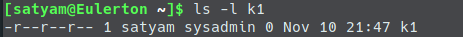
\includegraphics[width=10cm]{Ass62.png}
	\item  Give an example of clobbering and how to stop it.\\
Clobbering can be stopped by 	set -o noclobber
	\item What are the file permissions at the end of following commands?\\
	\$ umask 345\\
	\$ touch k1\\
	\$ chmod 436 k1\\
	\$ ls -l k1\\
	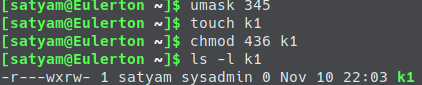
\includegraphics[width=10cm]{Ass63.png}
	\item  If you want to create a file “-xyz”, which command you should use?\\
 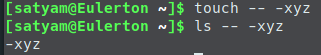
\includegraphics{Ass64.png}
	\item If a file has 000 permissions, then a root can .........the file. (read and/or write
	and/or execute )
	
	\item Which default permissions do you need to open a directory?\\
	Default permission should be read.
	\item If you want to add a sticky bit to the file, which command do you use? Example.
	\item Give examples of different filesystems.\\
ext4, ext3, FAT, NTFS,
	\item What is the starting point of the filesystem in Linux?\\
	Starting point of Linux filesystem is /
	\item What is absolute pathname?
	\\An absolute pathname, also referred to as an absolute path or a full path, is the location of a filesystem object (i.e., file, directory or link) relative to the root directory. 
	\item What is relative pathname?\\A reative pathname does not begin with a slash ( / ). Generally you specifies location relative to your current working directory. 
	\item If a filename has a space in it, which command-line option is used to access the file?\\
	Use Quotes or \ for spaces in filenames. (e.g., mkdir Hello\ World, mkdir "Hello World")
	\item Which command is used to unmount a filesystem?\\
	umount
	\item Why the df command is used?\\
	The df command is used to show the amount of disk space that is free on file systems.  This default action is to display used and free file space in blocks.
	\item Commands of Linux operating system reside in which directory?
	\item Which directory of Linux stores the Linux kernel?
	\\/lib: The Lib directory contains kernel modules and shared library images required to boot the system 
\item  Which directory of Linux stores the device drives?
\\/dev : Contains device files for all the hardware devices on the machine
\item  Which directory of Linux stores the configuration files?\\
/etc : Contains Application’s configuration files, startup, shutdown, start, stop script for every individual program.
\item  Which directory of Linux stores the information about running processes?\\
/proc : A virtual and pseudo file-system which contains information about running process with a particular Process-id aka pid.
\item Which directory of Linux is used as a default mount point of removable media?\\
/mnt : Temporary mount directory for mounting file system.
\item Which directory of Linux is a home of the superuser?\\
/root : This is the home directory of root(or super) user 
\item  What is the difference between locate and find command?\\
find searches in the real system. Is slower but always up-to-date and has more options (size, modification time,...)
\par
locate uses a previously built database (command updatedb). Is much faster, but uses an 'older' database and searches only names or parts of them.
\item  If you type find, what will be the output?\\
This command will search for files in a directory hierarchy. If no starting-point is
specified, `.' is assumed.


\item  If you type find ., what will be the output?\\
Prints a list of files in the current working directory.
\\ It will search all the files and directory to
\item  How many types of files are available in Linux OS?
	Regular files\\
Directories\\
Character device files\\
Block device files\\
Local domain sockets\\
Named pipes (FIFOs)\\
Symbolic links
\item  Which character/symbol is used to represent a regular file in the output of ls -l
command?\\
Hyphen(-) represents regular file in the output of ls -l
command
\item Which character/symbol is used to represent a directory in the output of ls -l command?
Symbol d represents a directory in the output of ls -l command
\item  Which character/symbol is used to represent a character device file in the output of
ls -l command?\\
Symbol c is  used to represent a character device file in the output of
ls -l command
\item  Which character/symbol is used to represent a block device file in the output of
ls -l command?\\
Symbol b is  used to represent a character device file in the output of
ls -l command
\item  Which character/symbol is used to represent a named pipes in the output of ls -l
command?\\
Symbol p is  used to represent a character device file in the output of
ls -l command
\item Which character/symbol is used to represent a symbolic link in the output of ls -l
command?\\
Symbol l is  used to represent a character device file in the output of
ls -l command
\item  Which command is used to create a directory?\\
mkdir [option] <directory-name(s)>
\item  Which command is used to create a symbolic link?\\
ln -s
\item What is the meaning of -- before the filename?\\
-- indicates that everything follows is a filename and not an option.
\item  Why the inode data structure is used?
\item Why the stat command is used?\\
It is preferred when viewing the inode
information of any individual file(s).
\item Which are the time related attributes available in inode?
\item  Which command do you use to create a hard link?\\
ln $<$file-name$>$ $<$link-name$>$
\item  Which command is used to view the total number of hard links of a file?\\
ls -l
\item In Linux, what is the meaning of . symbol?\\
The “.” refers to the current directory.

\item In Linux, what is the meaning of .. symbol?\\
The “..” refers to the parent directory.
\item What is the difference between a hard link and a symbolic link?
\item How many links are created by default, when we create a directory?\\
2 links are created by default
\item List at least one command/file-name (except passwd) which has setuid/setgid bit
set.
\end{enumerate}
\end{document}